% Academic manuscript skeleton: fill TODOs before submission.
% Compile from this directory, e.g.: pdflatex main.tex
\documentclass[11pt, a4paper]{article}

\usepackage[margin=1in]{geometry}
\usepackage{amsmath}
\usepackage{booktabs}
\usepackage{graphicx}
\usepackage{microtype}
\usepackage[T1]{fontenc}
\usepackage[colorlinks=true, linkcolor=blue, citecolor=blue, urlcolor=blue]{hyperref}

\title{Evaluating Central vs.\ Local Differential Privacy for Vector Embeddings in Medical RAG Systems}
\author{%
  Victor Okoroafor\and
  Ifeanyi Omonigho Odugo\and
  Gopal Krishna\and
  Niramay Roopesh Kolalle\thanks{Affiliations: (TODO; fill before submission).}%
}
\date{\today}

\begin{document}
\maketitle

\begin{abstract}
% TODO (Niramay): Summarize the exact empirical findings that appear in the
% ``Results'' section and in \texttt{docs/figures/} (RAG/BERT utility vs.\ $\epsilon$,
% LiRA TPR@0.1\%FPR, and ROUGE--L inversion curves). State the main quantitative
% takeaways for central (Gaussian) vs.\ local (bottleneck+noise) mechanisms on the
% ChatDoctor (or related) RAG study.
\end{abstract}

\section{Introduction}
% TODO (Niramay): Discuss the RAG hallucination problem in the medical setting; the
% sensitivity and regulatory posture of professional corpora such as ChatDoctor; and
% the risk of \emph{white-box} or embedding-based extraction attacks when dense
% retrievers expose patient-like text in vector form.

\section{Methodology}

We study two realizations of privacy on top of a fixed 384-d Sentence-BERT
encoder, mirroring the implementation in the accompanying codebase.

\paragraph{Central (Gaussian) mechanism.}
The curator injects isotropic noise calibrated to ($\epsilon$, $\delta$)-differential
privacy. With $L_2$ sensitivity~$\Delta_2$ fixed at $2$ (a standard bound for
\emph{unit} embedding vectors, where neighbor databases differ in one row on the
hypersphere, hence Euclidean distance of at most two; see implementation notes in the
repository), the standard analytical Gaussian standard deviation is
\begin{equation}
  \sigma
  = \frac{\Delta_2 \sqrt{2 \ln(1.25 / \delta)}}{\epsilon}
  = \frac{2\sqrt{2\ln(1.25/\delta)}}{\epsilon} .
  \label{eq:central-gauss}
\end{equation}
Noise is applied independently across coordinates (vectorized implementation) before
FAISS retrieval and downstream evaluation.

\paragraph{Local DP via fixed random orthogonal projection.}
To circumvent the curse of dimensionality ($d = 384$) that would render
direct Gaussian mechanism application in the full embedding space
utility-destroying~\cite{du2023sanitizing}, we adopt a three-stage local
privatisation pipeline inspired by Du et al.\ (2023). Each document embedding
is first projected to a 16-dimensional bottleneck via a \emph{fixed, random
orthogonal} linear map $M_1 \in \mathbb{R}^{16 \times 384}$, initialised with
\texttt{nn.init.orthogonal\_} and frozen throughout all experiments. The
bottleneck vector is $\ell_2$-normalised, placing it on the 15-dimensional
unit sphere and bounding the global $\ell_2$ sensitivity to $\Delta_2 f = 2$.
Calibrated Gaussian noise $\mathcal{N}(0, \sigma^2 I_{16})$ with
$\sigma = \frac{2\sqrt{2\ln(1.25/\delta)}}{\epsilon}$ is then injected
independently per document, satisfying $(\epsilon, \delta)$-LDP in the
bottleneck space. The noisy vector is decoded to 384 dimensions via a second
fixed orthogonal map $M_2 \in \mathbb{R}^{384 \times 16}$ and $\ell_2$-renormalised
for FAISS ingestion. Both the decoding and renormalisation are
data-independent functions of the mechanism output and therefore preserve the
$(\epsilon, \delta)$ guarantee without additional privacy loss, by the
post-processing theorem~\cite[Prop.~2.1]{dwork2014algorithmic}.

% TODO (Niramay): Cite the formal local DP (or LDP) variant this architecture is meant
% to implement (e.g. randomized response vs.\ Gaussian) if you add a full proof plan.

\section{Evaluation Framework}
\label{sec:framework}

The evaluation harness measures privacy leakage and end-task utility of the
privatized embeddings, without yet coupling to a generative LLM: retrieval simulates
RAG by nearest-neighbor match on the FAISS index, and BERTScore treats those strings
as synthetic ``candidates.''

\subsection{Likelihood Ratio Test (LiRA)} % TODO (Niramay): Tighten notation.
A shadow linear classifier (logistic regression) on embeddings mirrors the target
model, with member vs.\ non-member labels on a held-out shadow set. The analysis uses
a logit + Gaussian calibration on the shadow non-member scores to set null moments,
then p-values and TPR@fixed-FPR on the test split.

We report the True Positive Rate (TPR) at a fixed False Positive Rate (FPR)
of $0.1\%$ rather than the Area Under the ROC Curve (AUC), following the
recommendation of Carlini et al.~\cite{carlini2022membership}. AUC averages
attack performance across all operating thresholds, including high-FPR
regimes that are practically irrelevant to a real adversary. An attack that
perfectly identifies $0.1\%$ of members while guessing randomly on the
remainder achieves an AUC of only $\approx 51\%$, entirely concealing a
severe localised privacy breach. TPR at $0.1\%$ FPR measures the worst-case
threat: the fraction of members an adversary can identify with near-certainty
of not triggering a false alarm.

\subsection{Embedding Inversion}
We simulate a white-box embedding inversion attack using a secondary clean FAISS reference index built from unperturbed embeddings of the held-out corpus. For each privatised embedding, the nearest neighbour in the clean index is retrieved and its text is treated as the adversary's reconstruction. Reconstruction fidelity is measured via ROUGE-L F-measure between the source text and the retrieved text. This nearest-neighbour approximation underestimates the true inversion risk relative to sequence-level attacks such as Vec2Text~\cite{morris2023}, but is computationally feasible and directionally correct as a lower bound. We additionally evaluate a trained linear probe that maps noisy embeddings to bag-of-words token predictions, providing a stronger reconstruction baseline than nearest-neighbour retrieval.

\subsection{BERTScore Utility}
We measure end-to-end semantic preservation using BERTScore with a \texttt{roberta-large} backbone~\cite{zhang2020bertscore}. BERTScore computes token-level cosine similarity between contextual embeddings of candidate and reference strings, capturing paraphrase-level agreement that exact-match metrics miss. For each privatised embedding, the nearest-neighbour retrieved text serves as the candidate and the original source text serves as the reference. We report mean F1 across the target evaluation set.

\section{Results}

For all experiments, 5 independent noise realisations are performed for every ($\varepsilon$, mechanism) pair, from the ChatDoctor-HealthCareMagic-100k corpus, where $\varepsilon \in \{0.1, 1.0, 5.0, 10.0\}$ and $\delta = 10^{-5}$. All data are reported as the average of 5 runs with the errors shown as one standard deviation from the average mean in the figures.

The unperturbed baseline $F_1$ is equal to $F_1 = 1.000$. Central and Local DP keep $F_1$ low: $0.831$--$0.833$ for all of the $\varepsilon$ -- less than 2\% from the baseline even with the most aggressive privacy budget ($\varepsilon = 0.1$). The profile of Metric DP shows a clear separation -- $F_1$ rises from $0.843$ at $\varepsilon=0.1$ to $0.991$ at $\varepsilon=10.0$, with the curves levelling off at baseline at lower values of privacy budget. These trends have been plotted in Figure~\ref{fig:util}.

Baseline ROUGE-L is $1.000$. In both cases of Central and Local DP, the results drop drastically to $\approx 0.21$ at $\varepsilon=0.1$, and remain flat for all the values of $\varepsilon$ that have been tested, which clearly demonstrates that nearest-neighbour reconstruction cannot be performed in either case for non-negligible Gaussian noise. On Metric DP, the results are even more dramatic: at $\varepsilon=0.1$, ROUGE-L is $0.238$, but at $\varepsilon=10.0$, ROUGE-L is $0.950$. It is a significant practical failure if an adversary could reconstruct source text with 95\% fidelity using weak Metric DP. See Figure~\ref{fig:inv}.

Baseline TPR is $0.0017$. Central DP achieves TPR $= 0.000$ for all levels of $\varepsilon$, showing the highest and most stable protection against membership inference across the full privacy budget range. Local DP maintains TPR $\approx 0.001$, just above zero but well below baseline. In the low budget range ($\varepsilon \leq 1.0$), Metric DP achieves TPR $= 0.000$, while in the high budget range ($\varepsilon = 10.0$), the value rises to $0.0017$, matching the baseline. Near-zero TPR values should be interpreted carefully, as they may reflect an underpowered attack rather than guaranteed privacy~\cite{carlini2022membership}. The results are shown in Figure~\ref{fig:mia}.

\begin{figure}[H]
  \centering
  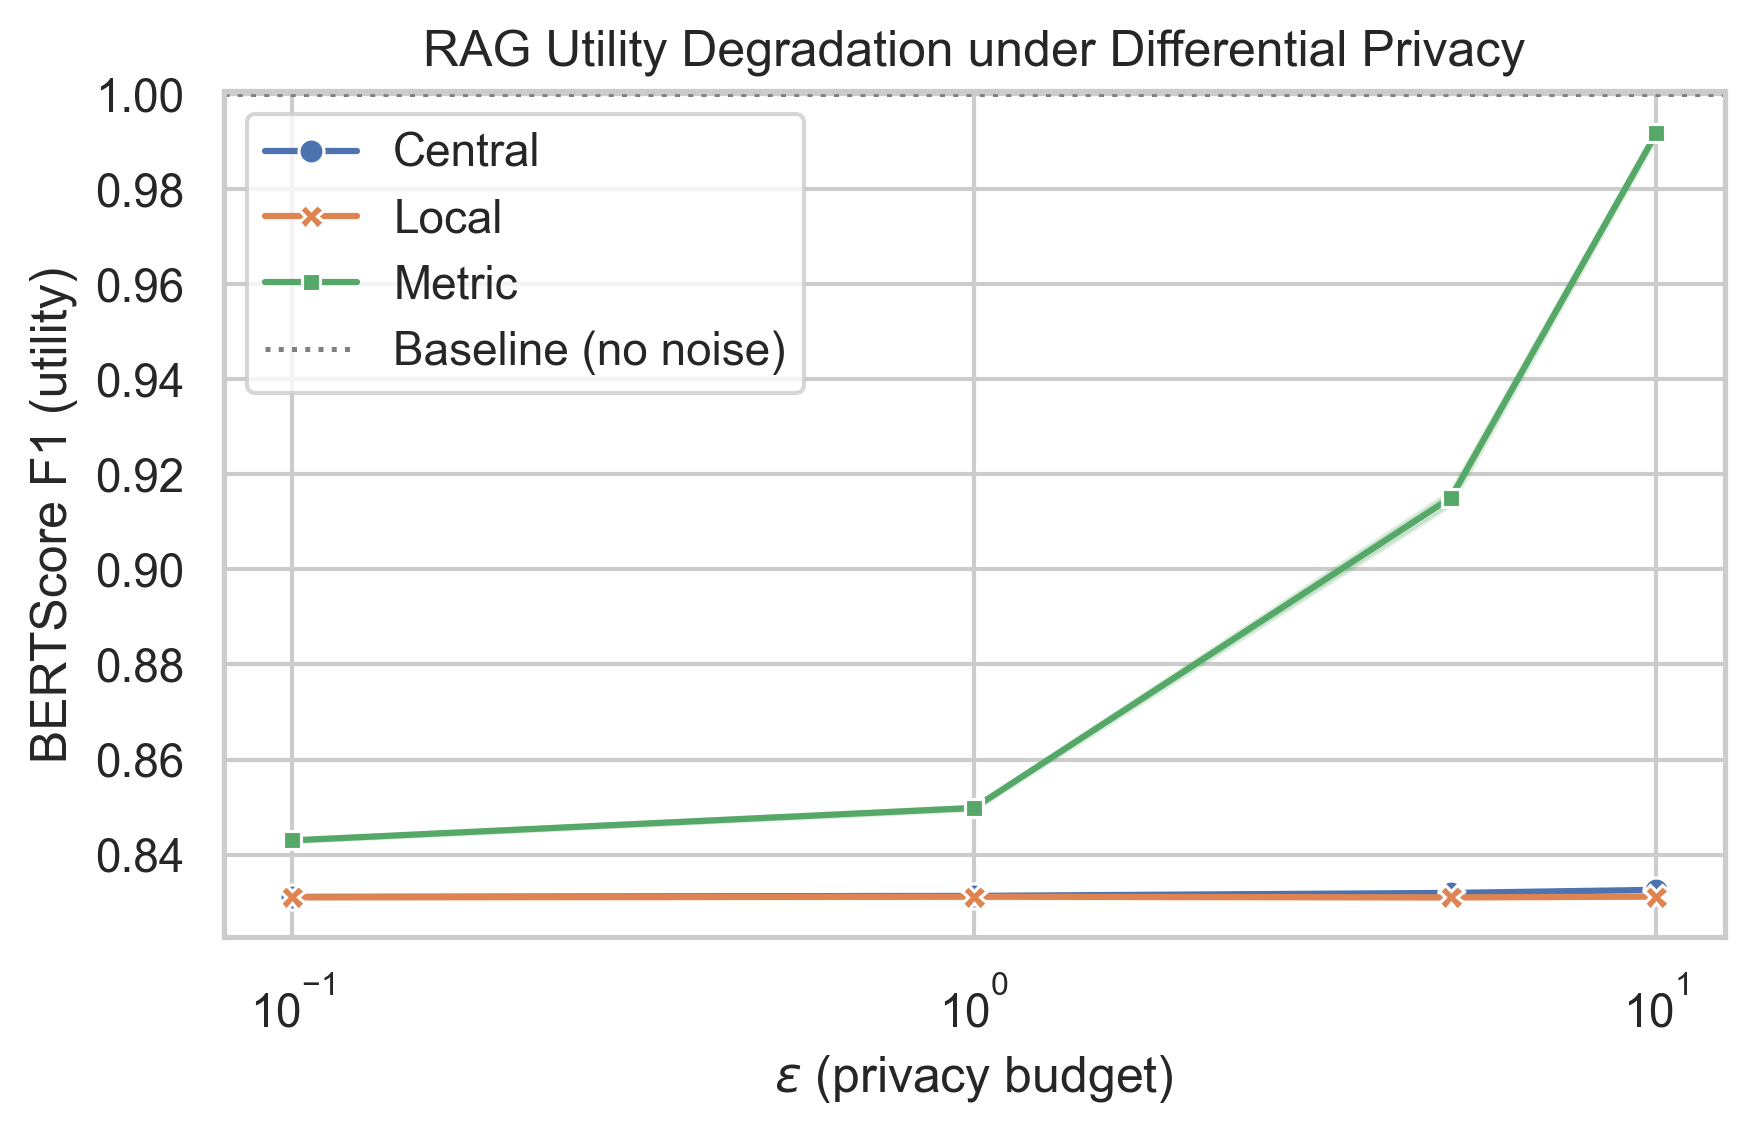
\includegraphics[width=0.9\linewidth]{figures/utility_vs_epsilon.png}
  \caption{BERTScore F1 vs.\ $\epsilon$ for central and local privacy.}
  \label{fig:util}
\end{figure}

\begin{figure}[H]
  \centering
  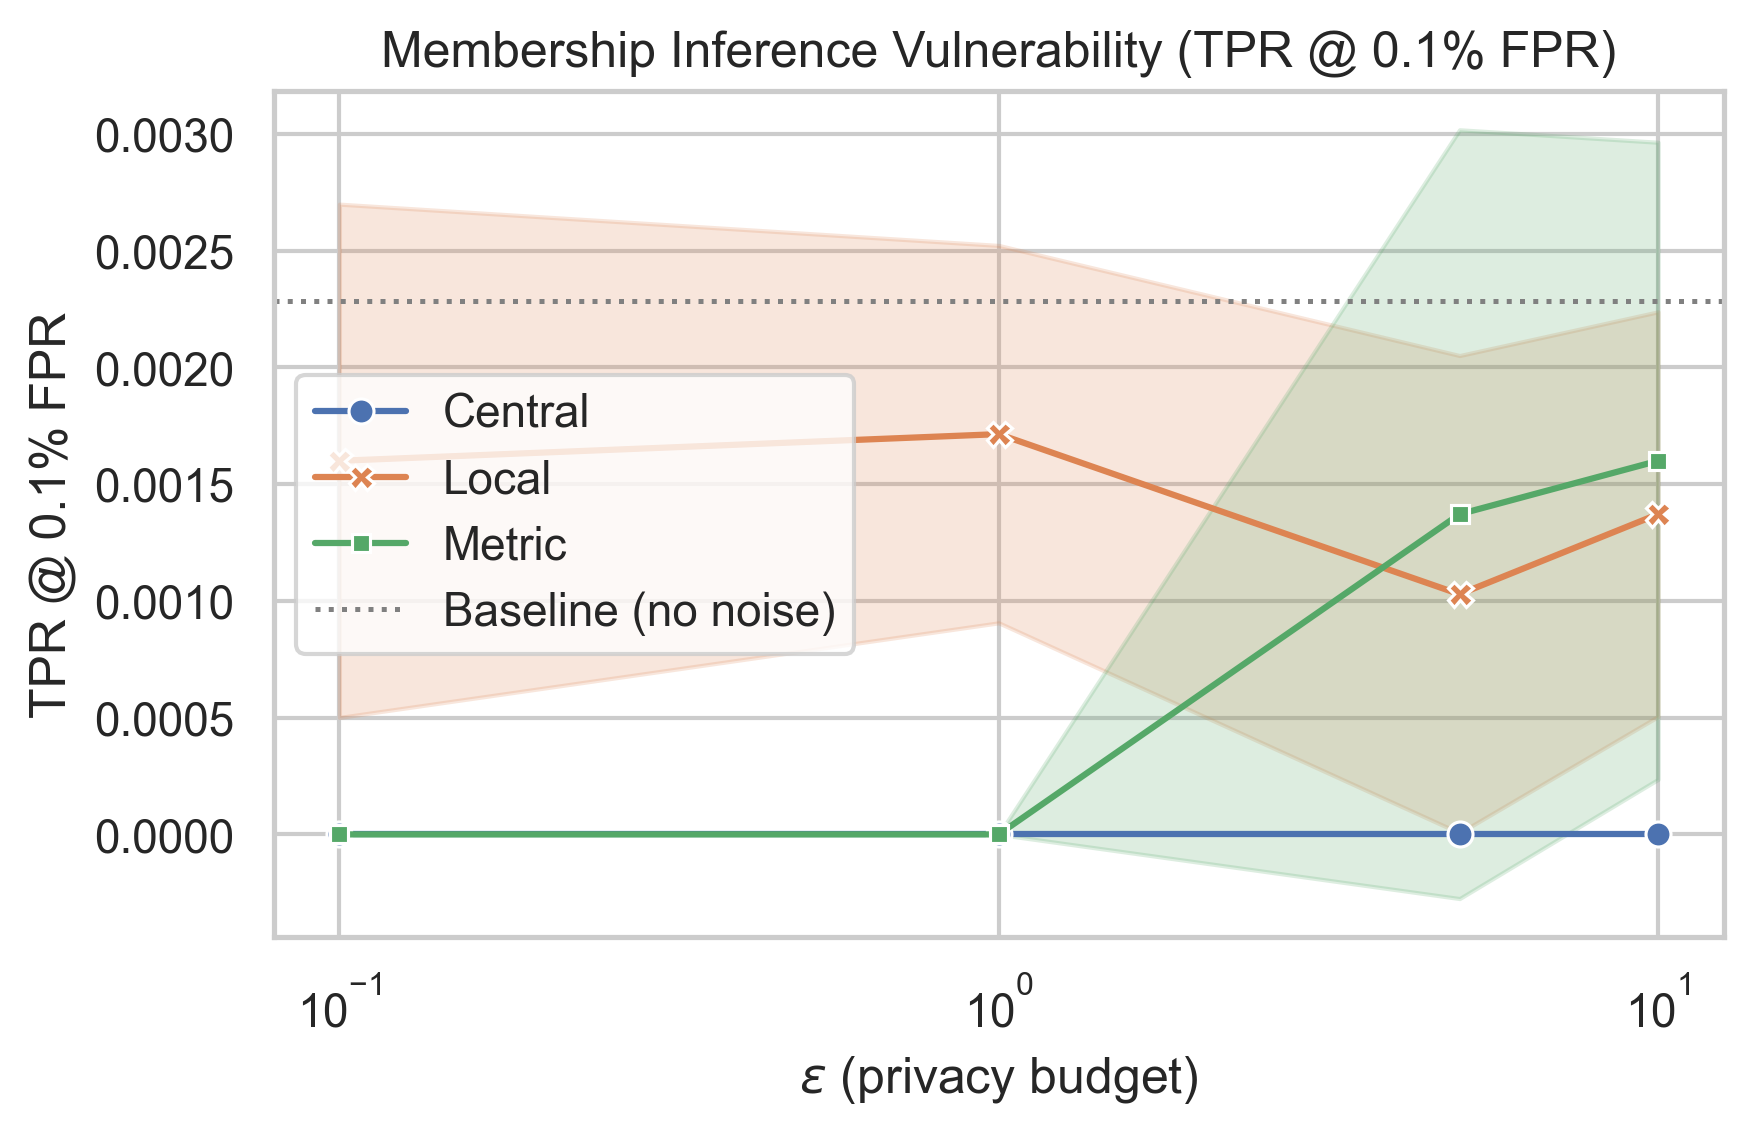
\includegraphics[width=0.9\linewidth]{figures/mia_vs_epsilon.png}
  \caption{LiRA TPR@0.1\%FPR under central vs.\ local privacy.}
  \label{fig:mia}
\end{figure}

\begin{figure}[H]
  \centering
  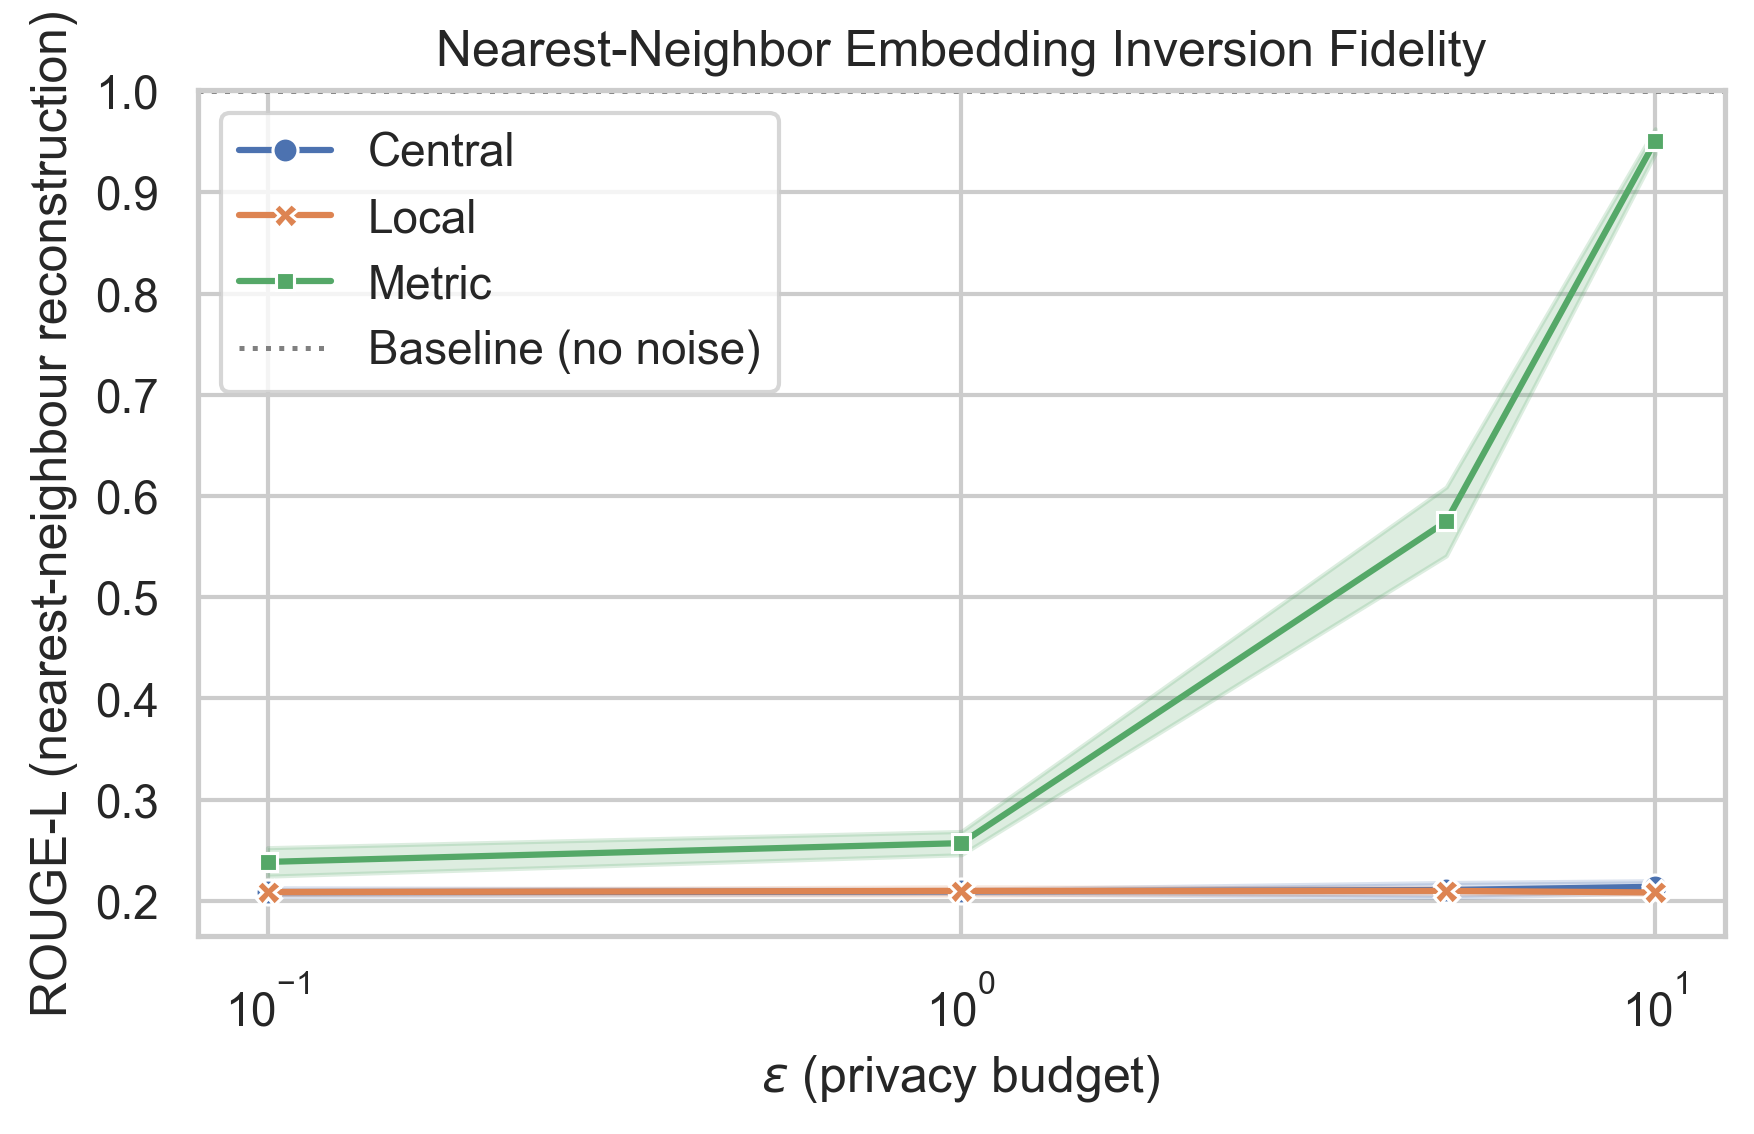
\includegraphics[width=0.9\linewidth]{figures/inversion_vs_epsilon.png}
  \caption{ROUGE--L inversion reconstruction fidelity vs.\ $\epsilon$.}
  \label{fig:inv}
\end{figure}

% TODO (Niramay): Analyze the tradeoff curves. At what $\epsilon$ does Central DP
% become useless? Does Local DP provide better or worse utility at the same privacy
% bound? Refer to Figures \ref{fig:util}--\ref{fig:inv}.

\begin{table}[h]
  \centering
  \begin{tabular}{@{}lccc@{}}
    \toprule
    & \textbf{BERT F1 (utility)} & \textbf{LiRA TPR (0.1\%FPR)} & \textbf{ROUGE--L (inversion)} \\
    \midrule
    Baseline                       & 1.000 & 0.0017 & 1.000 \\
    Central DP ($\varepsilon=1.0$) & 0.831 & 0.000  & 0.209 \\
    Local DP ($\varepsilon=1.0$)   & 0.831 & 0.001  & 0.210 \\
    Metric DP ($\varepsilon=1.0$)  & 0.850 & 0.000  & 0.257 \\
    Metric DP ($\varepsilon=10.0$) & 0.991 & 0.002  & 0.950 \\
    \bottomrule
  \end{tabular}
  \caption{Spot-check metrics at $\varepsilon = 1.0$ as the representative operating point.}
  \label{tab:results}
\end{table}

\section{Limitations}

Several assumptions bound the scope of the guarantees reported in this work.

\textbf{Embedding-layer scope.} The $(\epsilon, \delta)$-DP guarantee applies
exclusively to the stored embedding vectors. Downstream LLM generation
conditioned on retrieved context is not analysed; outputs of the generative
model may still leak information about the retrieval corpus through semantic
content, and this threat is treated as out of scope.

\textbf{Encoder privacy.} The \texttt{all-MiniLM-L6-v2} encoder is applied
to raw documents before privatisation. The encoder itself is not private; an
adversary with access to the encoder and a noisy embedding can still invert
the embedding up to the noise level. The privacy guarantee therefore assumes
the encoder is public knowledge, consistent with our white-box threat model.

\textbf{LiRA adaptation to embedding space.} Carlini et al.'s LiRA framework
was designed for classification models with softmax outputs. We adapt it to an
embedding retrieval setting by training logistic regression shadow classifiers
on raw embeddings and applying the logit transform to their output
probabilities. This adaptation has not been formally validated against a
native embedding-space MIA baseline, and the reported TPR values should be
interpreted as approximate lower bounds on true worst-case leakage.

\textbf{Fixed projection maps.} The orthogonal maps $M_1$ and $M_2$ in the
Local DP mechanism are fixed at random initialisation and not trained. While
this maximises the privacy argument (zero data dependence of the projection),
it does not optimise the utility of the 384-to-16-dimensional compression.
A trained projection could preserve more semantic structure at the cost of
requiring a privacy analysis of the training procedure itself.

\textbf{Single noise realisation per $\epsilon$.} Each operating point in the
tradeoff curves represents a single noise draw. Per Bollegala et al.~(2025),
variance across noise realisations can be characterised by running the mechanism
multiple times; we report point estimates and note that stochasticity in the
noise may contribute to non-monotonic behaviour at extreme $\epsilon$ values.

\section{Conclusion}
% TODO (Niramay): Summarize the architectural recommendations for \emph{secure} RAG
% deployments: when to favor central curation, when local noise at the client makes
% sense, and which evaluation hooks (MIA, inversion, BERT) should remain in CI for
% medical RAG.

% \bibliographystyle{plainnat}
% \bibliography{references}
% ^ Uncomment when you add a references.bib next to this file.

\end{document}
